\chapter{Clasificación de los grupos de alumnos según su rendimiento}\label{sec:chapterXIII}
\addcontentsline{toc}{chapter}{Clasificación de los grupos de alumnos según su rendimiento}

Para realizar la identificación de los subconjuntos de alumnos definidos en la Sección \ref{sec:badstudents}, se empleará el algoritmo de clasificación de Quinlan C5.0 \cite{Quinlan:See5C5}, que no es más que una herramienta de aprendizaje supervisado que genera un árbol de decisión o un conjunto de reglas. Así pues, las distintas categorías en las que se clasificarán a los grupos vendrán dadas en las hojas de dichos árboles y en los consecuentes de las reglas respectivamente. El clasificador estadístico C5.0 se basa en el concepto de entropía, seleccionando primero aquellas características cuyos valores se diferencian más entre distintas categorías de grupos de alumnos.

Se utilizarán como variables de entrada del clasificador tanto las medidas clásicas de rendimiento presentadas en el Capítulo \ref{chapter:rendimiento} como las medidas grafo-teóricas (Sección \ref{sec:complexity}). Por su parte, como categorías de salida, tendremos tanto una única partición en alumnos ``LOW'', que se supone que requieren más esfuerzo para superar el laboratorio, como las cinco particiones que se muestran en la Figura \ref{fig:KMeans5}.

Dado que hay muy pocos registros ($77$ en cada nivel), el problema de clasificación va a ser difícil y, con el fin de aumentar las evidencias requeridas por C5.0 para trabajar, el conjunto de datos se agrupará cada tres niveles consecutivos. Así pues, por un lado, agruparemos los niveles $3$, $4$ y $5$ para realizar predicciones al principio de la práctica y, por otro lado, agruparemos los niveles $8$, $9$ y $10$. Así pues, las siguientes secciones se dividirán en dos subapartados, dependiendo de la parte del dataset que estemos utilizando para entrenar el clasificador.

\section{Clasificación en grupos \emph{``LOW''} y \emph{``GOOD''}}

\subsection{Clasificación empleando las métricas clásicas de rendimiento}

\subsubsection{Clasificación empleando los niveles 8, 9 y 10}

Como podemos ver en la Figura \ref{fig:cmend1}, C5.0 obtiene un conjunto de reglas capaz de clasificar exactamente los $36$ grupos de tipo \emph{``LOW''} empleando los datos del último tercio del tiempo dedicado a la práctica, con un $p$ value $p < 2.2e-16$ estadísticamente muy relevante (Figura \ref{fig:cmend1}). Adicionalmente, las reglas para clasificar cada uno de los grupos obtenidas (Cuadro \ref{rulesend1}) son fácilmente interpretables. Por ejemplo, la regla $4$ nos indicaría que un grupo está en riesgo si no ha resuelto todos los problemas y tarda mucho en resolverlos una vez abiertos por primera vez.

\begin{figure}[H]
\centering
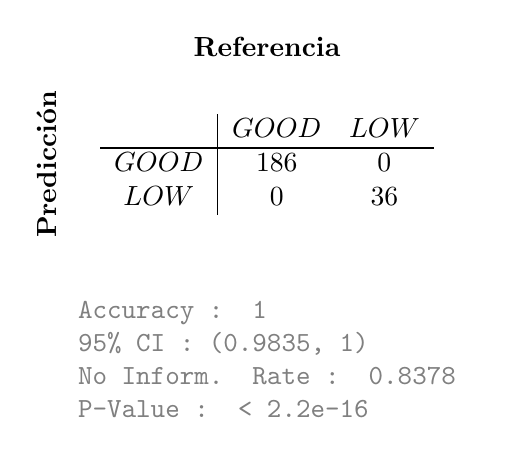
\begin{tikzpicture}
  \node (matrix)  {$\begin{array}{c|cc}
			 & GOOD & LOW \\ \hline
        GOOD & 186  & 0 \\
        LOW & 0 & 36
\end{array}$};
  \node[above of= matrix, node distance=0.5cm, yshift=1cm,font=\color{black}] {\textbf{Referencia}};
  \node[left of= matrix, node distance=3.5cm, rotate=90, anchor=center,yshift=-0.7cm,font=\color{black}] {\textbf{Predicción}};
  % Tabular environment for additional text
  \node[below of=matrix, node distance=2.5cm,font=\color{gray}]{
    \begin{tabular}{l}
      \texttt{Accuracy : 1} \\
      \texttt{95\% CI : (0.9835, 1)} \\
      \texttt{No Inform. Rate : 0.8378} \\
      \texttt{P-Value : < 2.2e-16}
    \end{tabular}
  };
\end{tikzpicture}
\caption{Aprendiendo a identificar a los grupos \emph{``LOW''}, es decir, aquellos con una puntuación inferior a $8.1$ sobre $10$.}
\label{fig:cmend1}
\end{figure}

\begin{tcolorbox}[title=Reglas de clasificación para identificar grupos de tipo \emph{``LOW''}.]
  %add special color box to list of listings
  \makeatletter
  \addcontentsline{lol}{subsection}{\kvtcb@title}
  \makeatother
\begin{multicols}{2}
    \begin{minted}{R}
Rule 75/1: (73.8, lift 1.4)
	ns > 0.342623
	rt > 0.01037344
	rt <= 0.3019366
	sq > 0.8140351
	->  class GOOD  [0.987]

Rule 75/2: (22.9, lift 1.4)
	np > 0.8888889
	rt > 0.3019366
	->  class GOOD  [0.960]

Rule 75/3: (50.4/4, lift 1.3)
	np <= 0.8888889
	rt <= 0.3676471
	->  class GOOD  [0.905]

Rule 75/4: (5.3, lift 2.9)
	np <= 0.8888889
	rt > 0.3676471
	->  class LOW  [0.864]

Rule 75/5: (5.2, lift 2.9)
	np > 0.8888889
	rt <= 0.3019366
	sq <= 0.8140351
	->  class LOW  [0.861]

Rule 75/6: (11.4/1.3, lift 2.8)
	ns > 0.342623
	np > 0.8888889
	rt <= 0.01037344
	->  class LOW  [0.831]

Rule 75/7: (70.1/28.1, lift 2.0)
	ns <= 0.342623
	np > 0.8888889
	rt <= 0.3019366
	->  class LOW  [0.596]
	
Default class: GOOD
    \end{minted}
  \end{multicols}
\label{rulesend1}
\end{tcolorbox}

\subsubsection{Clasificación empleando los niveles 3, 4 y 5}

Como podemos ver en la Figura \ref{fig:cmbegin1}, C5.0 no es capaz de identificar a los grupos en riesgo empleando sólo las medidas clásicas de rendimiento a partir de los datos de los niveles $3$, $4$ y $5$. Si observamos el Cuadro \ref{rulesbegin1}, vemos que se establece que todos los grupos se clasifican como de tipo \emph{``GOOD''} por defecto.

\begin{figure}[H]
\centering
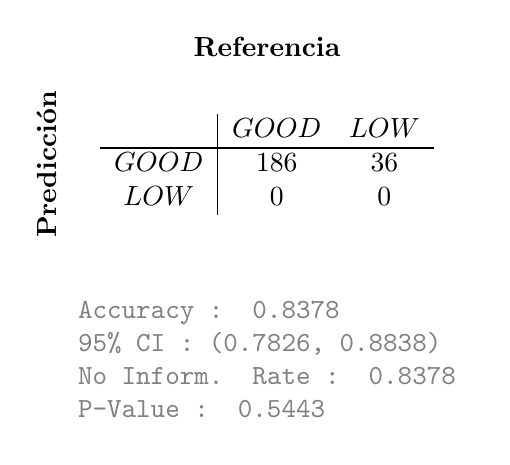
\begin{tikzpicture}
  \node (matrix)  {$\begin{array}{c|cc}
			 & GOOD & LOW \\ \hline
        GOOD & 186  & 36 \\
        LOW & 0 & 0
\end{array}$};
  \node[above of= matrix, node distance=0.5cm, yshift=1cm,font=\color{black}] {\textbf{Referencia}};
  \node[left of= matrix, node distance=3.5cm, rotate=90, anchor=center,yshift=-0.7cm,font=\color{black}] {\textbf{Predicción}};
  % Tabular environment for additional text
  \node[below of=matrix, node distance=2.5cm,font=\color{gray}]{
    \begin{tabular}{l}
      \texttt{Accuracy : 0.8378} \\
      \texttt{95\% CI : (0.7826, 0.8838)} \\
      \texttt{No Inform. Rate : 0.8378} \\
      \texttt{P-Value : 0.5443}
    \end{tabular}
  };
\end{tikzpicture}
\caption{Aprendiendo a identificar a los grupos \emph{``LOW''}, es decir, aquellos con una puntuación inferior a $8.1$ sobre $10$.}
\label{fig:cmbegin1}
\end{figure}

\begin{tcolorbox}[title=Reglas de clasificación para identificar grupos de tipo \emph{``LOW''}.]
  %add special color box to list of listings
  \makeatletter
  \addcontentsline{lol}{subsection}{\kvtcb@title}
  \makeatother
\begin{multicols}{2}
    \begin{minted}{R}
Default class: GOOD
    \end{minted}
  \end{multicols}
\label{rulesbegin1}
\end{tcolorbox}

Pero no sólo esto, ¿podríamos dar un gran paso y predecir no sólo equipos \emph{``LOW''}/\emph{``GOOD''}, sino también un límite inferior y superior de sus calificaciones finales, y adivinar en cuál de los $5$ intervalos de la Figura \ref{fig:KMeans5} se encuentran? La respuesta es, felizmente, sí (Sección \ref{sec:intervals}).

\subsection{Clasificación empleando una combinación de todas las métricas}

A continuación, se repetirán los experimentos anteriores, pero ahora empleando las funciones $np$, $fr$, $ps$, $sq$, $Cl$, $De$, $Dm$, $Le$, $Di$, $We$, $Ef$, $St$, $Dag$, $WDag$, $Be$ y $Ba$.

\subsubsection{Clasificación empleando los niveles 8, 9 y 10}

El resultado es que C5.0 obtiene un conjunto de reglas capaz de clasificar exactamente los $36$ casos de grupos \emph{``LOW''} del nivel $8$ en adelante, es decir, a partir del último tercio del periodo de tiempo dedicado a la práctica, con un $p$ value $p < 2.2e-16$ estadísticamente muy relevante (Figura \ref{fig:cm4}). Las reglas obtenidas pueden consultarse en el Cuadro \ref{rules4}.

\begin{figure}[H]
\centering
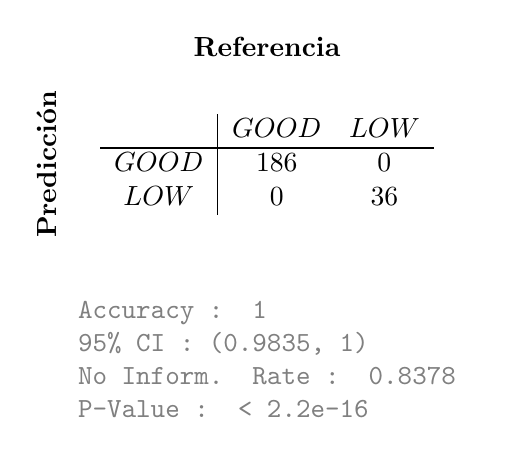
\begin{tikzpicture}
  \node (matrix)  {$\begin{array}{c|cc}
			 & GOOD & LOW \\ \hline
        GOOD & 186  & 0 \\
        LOW & 0 & 36
\end{array}$};
  \node[above of= matrix, node distance=0.5cm, yshift=1cm,font=\color{black}] {\textbf{Referencia}};
  \node[left of= matrix, node distance=3.5cm, rotate=90, anchor=center,yshift=-0.7cm,font=\color{black}] {\textbf{Predicción}};
  % Tabular environment for additional text
  \node[below of=matrix, node distance=2.5cm,font=\color{gray}]{
    \begin{tabular}{l}
      \texttt{Accuracy : 1} \\
      \texttt{95\% CI : (0.9835, 1)} \\
      \texttt{No Inform. Rate : 0.8378} \\
      \texttt{P-Value : < 2.2e-16}
    \end{tabular}
  };
\end{tikzpicture}
\caption{Aprendiendo a identificar a los grupos \emph{``LOW''}, es decir, aquellos con una puntuación inferior a $8.1$ sobre $10$.}
\label{fig:cm4}
\end{figure}

\begin{tcolorbox}[title=Reglas de clasificación para identificar grupos de tipo \emph{``LOW''}.]
  %add special color box to list of listings
  \makeatletter
  \addcontentsline{lol}{subsection}{\kvtcb@title}
  \makeatother
\begin{multicols}{2}
    \begin{minted}[fontsize=\footnotesize]{R}
Rule 99/1: (44.4, lift 1.5)
	sq > 0.9719298
	Di > -8.39991
	We > 0.1196341
	Ef > 7
	St > 3.988984
	St <= 15.42027
	->  class GOOD  [0.978]

Rule 99/2: (27.8, lift 1.4)
	St <= 15.42027
	Ba <= 5.436692
	->  class GOOD  [0.966]

Rule 99/3: (25.9, lift 1.4)
	We > 0.7189189
	->  class GOOD  [0.964]

Rule 99/4: (41/0.8, lift 1.4)
	sq <= 0.9411765
	St <= 15.42027
	->  class GOOD  [0.958]

Rule 99/5: (64.1/2.7, lift 1.4)
	fr > 0.04813478
	Di > -8.39991
	We > 0.1196341
	Ef > 7
	St > 3.988984
	St <= 15.42027
	Be <= 5
	->  class GOOD  [0.944]

Rule 99/6: (10, lift 1.4)
	St <= 15.42027
	Be > 6
	->  class GOOD  [0.917]

Rule 99/7: (7.7, lift 1.3)
	St <= 1.791759
	->  class GOOD  [0.897]

Rule 99/8: (8.5, lift 2.7)
	fr <= 0.04813478
	sq > 0.9411765
	sq <= 0.9719298
	Ba > 5.436692
	->  class LOW  [0.905]

Rule 99/9: (8, lift 2.7)
	sq > 0.9411765
	sq <= 0.9719298
	St > 3.988984
	Be > 5
	Be <= 6
	Ba > 5.436692
	->  class LOW  [0.900]

Rule 99/10: (6.7, lift 2.7)
	We <= 0.1196341
	St > 3.988984
	->  class LOW  [0.885]

Rule 99/11: (8.1/0.2, lift 2.7)
	sq > 0.9411765
	Ef <= 7
	->  class LOW  [0.878]

Rule 99/12: (27.4/3.3, lift 2.6)
	St > 1.791759
	St <= 3.988984
	Be <= 6
	Ba > 5.436692
	->  class LOW  [0.853]

Rule 99/13: (15.1/1.8, lift 2.5)
	We <= 0.7189189
	St > 15.42027
	->  class LOW  [0.834]

Rule 99/14: (14.4/3.1, lift 2.3)
	sq > 0.9411765
	Di <= -8.39991
	We <= 0.7189189
	St <= 15.42027
	Ba > 5.436692
	->  class LOW  [0.752]
	
Default class: GOOD
    \end{minted}
  \end{multicols}
\label{rules4}
\end{tcolorbox}

\subsubsection{Clasificación empleando los niveles 3, 4 y 5}

El resultado es que C5.0 obtiene un conjunto de reglas capaz de clasificar exactamente $35$ de los $36$ casos de grupos \emph{``LOW''} del nivel $3$ en adelante, es decir, a partir de un tercio del periodo de tiempo dedicado a la práctica, con un $p$ value $p = 3.843e-16$ estadísticamente muy relevante (Figura \ref{fig:cm1}). Entre las reglas obtenidas (Cuadro \ref{rules1}), la regla $4$ dice: ``Un grupo no está en riesgo si ha realizado muchas sesiones (\texttt{We > 0.3286957})''. O la regla $16$ que dice ``Un grupo está en riesgo si no ha seguido el orden que el profesor esperaba (\texttt{sq <= 0.9877296}), tiene pocas sesiones (\texttt{We <= 0.3286957}) y no se centra por igual en todos los problemas (\texttt{Ba > 6.715498})''. %Esto es como el mal gráfico mostrado al principio de este documento en la Figura 1, largo y desconectado.

\begin{figure}[H]
\centering
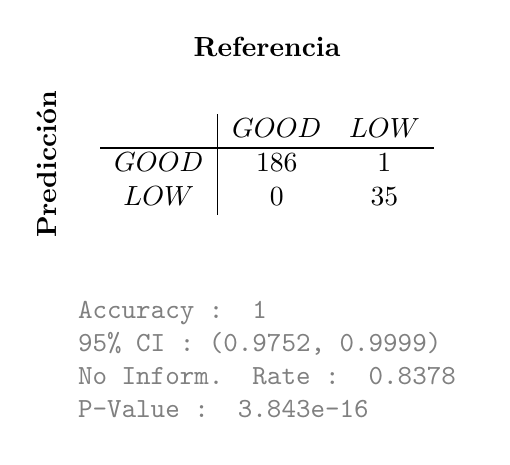
\begin{tikzpicture}
  \node (matrix)  {$\begin{array}{c|cc}
			 & GOOD & LOW \\ \hline
        GOOD & 186  & 1 \\
        LOW & 0 & 35
\end{array}$};
  \node[above of= matrix, node distance=0.5cm, yshift=1cm,font=\color{black}] {\textbf{Referencia}};
  \node[left of= matrix, node distance=3.5cm, rotate=90, anchor=center,yshift=-0.7cm,font=\color{black}] {\textbf{Predicción}};
  % Tabular environment for additional text
  \node[below of=matrix, node distance=2.5cm,font=\color{gray}]{
    \begin{tabular}{l}
      \texttt{Accuracy : 1} \\
      \texttt{95\% CI : (0.9752, 0.9999)} \\
      \texttt{No Inform. Rate : 0.8378} \\
      \texttt{P-Value : 3.843e-16}
    \end{tabular}
  };
\end{tikzpicture}
\caption{Aprendiendo a identificar a los grupos \emph{``LOW''}, es decir, aquellos con una puntuación inferior a $8.1$ sobre $10$.}
\label{fig:cm1}
\end{figure}

\begin{tcolorbox}[title=Reglas de clasificación para identificar grupos de tipo \emph{``LOW''}.]
  %add special color box to list of listings
  \makeatletter
  \addcontentsline{lol}{subsection}{\kvtcb@title}
  \makeatother
\begin{multicols}{2}
    \begin{minted}[fontsize=\scriptsize]{R}
Rule 4/1: (34.6, lift 1.4)
	Dm > 1.181818
	Ba <= 6.715498
	->  class GOOD  [0.973]

Rule 4/2: (31.7, lift 1.4)
	Cl > 0.2564103
	St > 1.098612
	Ba <= 6.715498
	->  class GOOD  [0.970]

Rule 4/3: (19, lift 1.4)
	fr <= 0.14
	sq > 0.9528306
	We <= 0.2347826
	Be <= 2
	->  class GOOD  [0.952]

Rule 4/4: (17.8, lift 1.4)
	We > 0.3286957
	->  class GOOD  [0.949]

Rule 4/5: (21.9/0.4, lift 1.4)
	sq <= 0.9036961
	Ba <= 6.715498
	->  class GOOD  [0.942]

Rule 4/6: (37.2/1.3, lift 1.4)
	Cl > 0.2564103
	We <= 0.2347826
	St > 0
	Ba <= 6.715498
	->  class GOOD  [0.941]

Rule 4/7: (14.8, lift 1.4)
	np <= 1.2
	sq > 0.9528306
	We <= 0.2347826
	Be <= 2
	Ba <= 6.715498
	->  class GOOD  [0.940]

Rule 4/8: (9.9, lift 1.3)
	We > 0.2018018
	We <= 0.2347826
	St <= 0
	->  class GOOD  [0.916]

Rule 4/9: (9.6, lift 1.3)
	ps <= 0.1484849
	sq > 0.9877296
	Ba > 6.715498
	->  class GOOD  [0.914]

Rule 4/10: (48.2/6.7, lift 1.2)
	Be > 2
	Ba <= 6.715498
	->  class GOOD  [0.846]

Rule 4/11: (7.2, lift 2.8)
	sq > 0.9036961
	Cl <= 0.2564103
	Dm <= 1.181818
	Be <= 2
	Ba <= 6.715498
	->  class LOW  [0.891]

Rule 4/12: (6.9, lift 2.8)
	ps > 0.1484849
	We <= 0.3286957
	Ba > 6.715498
	->  class LOW  [0.887]

Rule 4/13: (10.5/0.8, lift 2.7)
	sq > 0.9528306
	We > 0.2347826
	We <= 0.3286957
	St <= 1.098612
	Be <= 2
	Ba <= 6.715498
	->  class LOW  [0.860]

Rule 4/14: (7.1/1.6, lift 2.3)
	sq > 0.9036961
	sq <= 0.9528306
	St <= 1.098612
	Ba <= 6.715498
	->  class LOW  [0.717]

Rule 4/15: (27.4/8.8, lift 2.1)
	np > 1.2
	fr > 0.14
	We <= 0.2018018
	St <= 0
	Be <= 2
	->  class LOW  [0.667]

Rule 4/16: (24.4/8, lift 2.1)
	sq <= 0.9877296
	We <= 0.3286957
	Ba > 6.715498
	->  class LOW  [0.658]
	
Default class: GOOD
    \end{minted}
  \end{multicols}
\label{rules1}
\end{tcolorbox}

\subsection{Clasificación empleando las medidas de complejidad de propósito general}

\subsubsection{Clasificación empleando los niveles 8, 9 y 10}

El resultado es que C5.0 obtiene un conjunto de reglas capaz de clasificar exactamente los $36$ casos de grupos \emph{``LOW''} del nivel $8$ en adelante, es decir, a partir del último tercio del periodo de tiempo dedicado a la práctica, con un $p$ value $p < 2.2e-16$ estadísticamente muy relevante (Figura \ref{fig:cm3}). Además, las reglas obtenidas (Cuadro \ref{rules3}) tienen pleno sentido.

\begin{figure}[H]
\centering
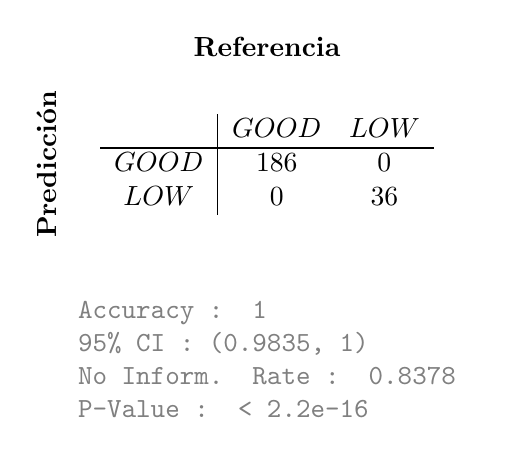
\begin{tikzpicture}
  \node (matrix)  {$\begin{array}{c|cc}
			 & GOOD & LOW \\ \hline
        GOOD & 186  & 0 \\
        LOW & 0 & 36
\end{array}$};
  \node[above of= matrix, node distance=0.5cm, yshift=1cm,font=\color{black}] {\textbf{Referencia}};
  \node[left of= matrix, node distance=3.5cm, rotate=90, anchor=center,yshift=-0.7cm,font=\color{black}] {\textbf{Predicción}};
  % Tabular environment for additional text
  \node[below of=matrix, node distance=2.5cm,font=\color{gray}]{
    \begin{tabular}{l}
      \texttt{Accuracy : 1} \\
      \texttt{95\% CI : (0.9835, 1)} \\
      \texttt{No Inform. Rate : 0.8378} \\
      \texttt{P-Value : < 2.2e-16}
    \end{tabular}
  };
\end{tikzpicture}
\caption{Aprendiendo a identificar a los grupos \emph{``LOW''}, es decir, aquellos con una puntuación inferior a $8.1$ sobre $10$.}
\label{fig:cm3}
\end{figure}

\begin{tcolorbox}[title=Reglas de clasificación para identificar grupos de tipo \emph{``LOW''}.]
  %add special color box to list of listings
  \makeatletter
  \addcontentsline{lol}{subsection}{\kvtcb@title}
  \makeatother
\begin{multicols}{2}
    \begin{minted}{R}
Rule 99/1: (8.3, lift 1.3)
	St <= 1.791759
	->  class GOOD  [0.903]

Rule 99/2: (8.3, lift 1.3)
	Be <= 1
	Ba <= 7.664816
	->  class GOOD  [0.903]

Rule 99/3: (81.3/11, lift 1.3)
	We > 0.4208696
	->  class GOOD  [0.855]

Rule 99/4: (72.7/13, lift 1.2)
	Cl <= 0.2771242
	We > 0.06390639
	We <= 0.4208696
	Be > 4
	->  class GOOD  [0.812]

Rule 99/5: (28.1/1.9, lift 2.8)
	We <= 0.4208696
	St > 1.791759
	Be <= 4
	Ba > 7.664816
	->  class LOW  [0.905]

Rule 99/6: (6.9, lift 2.7)
	Di > -8.386857
	St > 15.46906
	->  class LOW  [0.883]

Rule 99/7: (4.8, lift 2.6)
	Cl > 0.2771242
	Be > 4
	->  class LOW  [0.852]

Rule 99/8: (28.7/4.1, lift 2.6)
	We <= 0.4208696
	St > 1.791759
	Be > 1
	Be <= 4
	->  class LOW  [0.834]

Rule 99/9: (5.3/0.4, lift 2.5)
	We <= 0.06390639
	Be > 4
	->  class LOW  [0.815]

Default class: GOOD
    \end{minted}
  \end{multicols}
\label{rules3}
\end{tcolorbox}

\subsubsection{Clasificación empleando los niveles 3, 4 y 5}

El resultado es que C5.0 obtiene un conjunto de reglas capaz de clasificar exactamente $35$ de los $36$ casos de grupos \emph{``LOW''} del nivel $3$ en adelante, es decir, a partir de un tercio del periodo de tiempo dedicado a la práctica, con un $p$ value $p = 3.843e-16$ estadísticamente muy relevante (Figura \ref{fig:cm2}). Además, las reglas obtenidas (Cuadro \ref{rules2}) tienen pleno sentido. Por ejemplo, la regla $7$ dice: ``Un grupo está en riesgo si está centrado en los problemas con numeración alta (\texttt{Be > 6})''. O la regla $3$ que dice ``Un grupo está en riesgo si no se ha centrado por igual en todos los problemas (\texttt{Ba > 3.366005}) y recorre caminos menos largos en media (\texttt{WDag > -4.317488}) teniendo en cuenta que el valor de máxima probabilidad de la métrica $WDag$ es $-4.19$.

\begin{figure}[H]
\centering
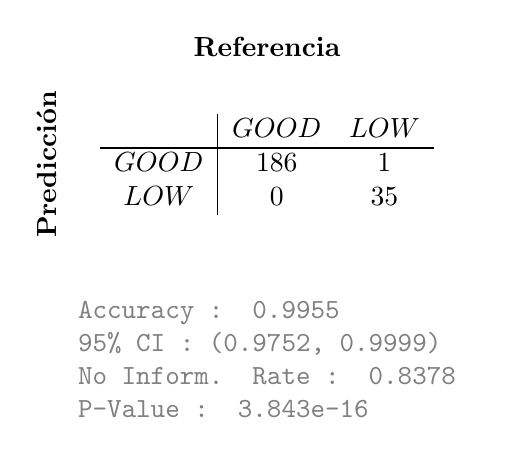
\begin{tikzpicture}
  \node (matrix)  {$\begin{array}{c|cc}
			 & GOOD & LOW \\ \hline
        GOOD & 186  & 1 \\
        LOW & 0 & 35
\end{array}$};
  \node[above of= matrix, node distance=0.5cm, yshift=1cm,font=\color{black}] {\textbf{Referencia}};
  \node[left of= matrix, node distance=3.5cm, rotate=90, anchor=center,yshift=-0.7cm,font=\color{black}] {\textbf{Predicción}};
  % Tabular environment for additional text
  \node[below of=matrix, node distance=2.5cm,font=\color{gray}]{
    \begin{tabular}{l}
      \texttt{Accuracy : 0.9955} \\
      \texttt{95\% CI : (0.9752, 0.9999)} \\
      \texttt{No Inform. Rate : 0.8378} \\
      \texttt{P-Value : 3.843e-16 }
    \end{tabular}
  };
\end{tikzpicture}
\caption{Aprendiendo a identificar a los grupos \emph{``LOW''}, es decir, aquellos con una puntuación inferior a $8.1$ sobre $10$.}
\label{fig:cm2}
\end{figure}

\begin{tcolorbox}[title=Reglas de clasificación para identificar grupos de tipo \emph{``LOW''}.]
  %add special color box to list of listings
  \makeatletter
  \addcontentsline{lol}{subsection}{\kvtcb@title}
  \makeatother
\begin{multicols}{2}
    \begin{minted}{R}
Rule 11/1: (17.8, lift 1.5)
	Ba > 9.26712
	->  class GOOD  [0.949]

Rule 11/2: (200.7/68.3, lift 1.0)
	De > 0.0952381
	->  class GOOD  [0.658]

Rule 11/3: (8.5/0.3, lift 2.5)
	WDag > -4.317488
	Ba > 3.366005
	->  class LOW  [0.880]

Rule 11/4: (5, lift 2.4)
	Dm <= 1.2
	Ef <= 4
	St > 1.791759
	->  class LOW  [0.858]

Rule 11/5: (8.3/0.6, lift 2.4)
	De <= 0.0989011
	Ef <= 4
	Ba <= 9.26712
	->  class LOW  [0.850]

Rule 11/6: (9.4/1.1, lift 2.3)
	De > 0.1153846
	Ef > 3
	Ef <= 4
	WDag <= -6.612041
	Ba > 3.366005
	->  class LOW  [0.818]

Rule 11/7: (3.4, lift 2.3)
	Be > 6
	->  class LOW  [0.814]

Rule 11/8: (13.3/2.3, lift 2.2)
	De <= 0.0952381
	Ba <= 9.26712
	->  class LOW  [0.783]

Rule 11/9: (19.9/5.4, lift 2.0)
	Dm <= 1.222222
	Ef <= 3
	St > 0.6931472
	Ba <= 9.26712
	->  class LOW  [0.707]

Default class: GOOD
    \end{minted}
  \end{multicols}
\label{rules2}
\end{tcolorbox}

\section{Clasificación en intervalos de notas}\label{sec:intervals}

\subsection{Clasificación empleando las métricas clásicas de rendimiento}

\subsubsection{Clasificación empleando los niveles 8, 9 y 10}

Como podemos ver en la Figura \ref{fig:cmend2}, C5.0 obtiene un conjunto de reglas (Cuadro \ref{rulesend2}) capaz de clasificar exactamente a todos los grupos dentro de su correspondiente intervalo de calificaciones a partir de los datos del último tercio del periodo de tiempo dedicado a la práctica, con un $p$ value $p < 2.2e-16$ estadísticamente muy relevante (Figura \ref{fig:cmend2}).

\begin{figure}[H]
\centering
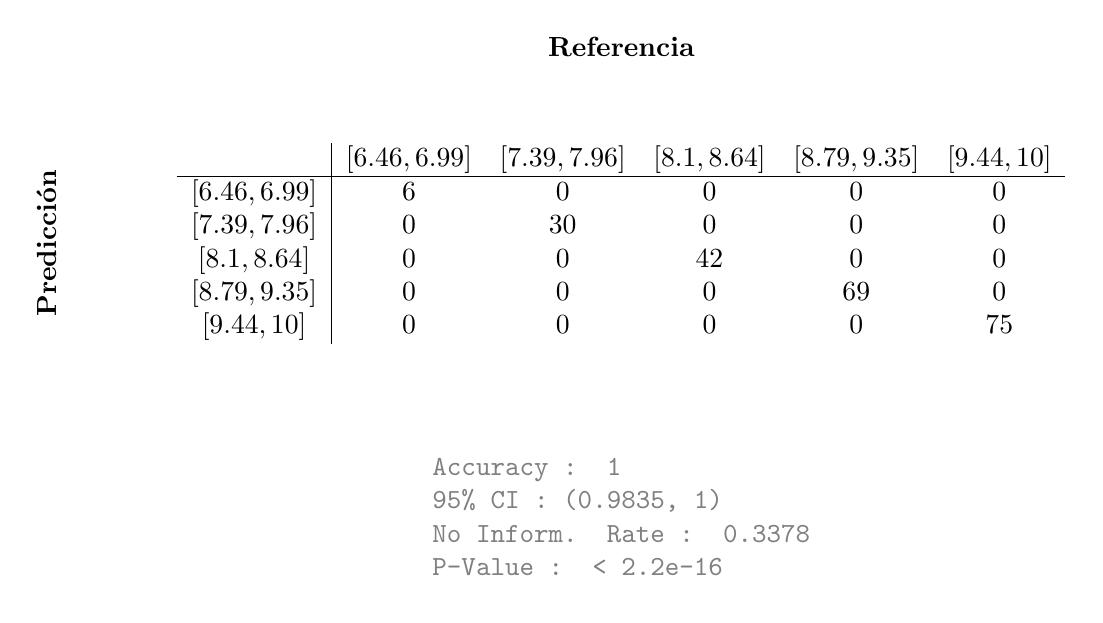
\begin{tikzpicture}
  \node (matrix)  {$\begin{array}{c|ccccc}
                         & \left[6.46,6.99\right] & \left[7.39,7.96\right] & \left[8.1,8.64\right] & \left[8.79,9.35\right] & \left[9.44,10\right]\\ \hline
        \left[6.46,6.99\right] & 6 & 0 & 0 & 0 & 0 \\
        \left[7.39,7.96\right] & 0 & 30 & 0 & 0 & 0 \\
        \left[8.1,8.64\right] & 0 & 0 & 42 & 0 & 0 \\
        \left[8.79,9.35\right] & 0 & 0 & 0 & 69 & 0 \\
        \left[9.44,10\right] & 0 & 0 & 0 & 0 & 75
\end{array}$};
  \node[above of= matrix, node distance=1.5cm, yshift=1cm,font=\color{black}] {\textbf{Referencia}};
  \node[left of= matrix, node distance=8cm, rotate=90, anchor=center,yshift=-0.7cm,font=\color{black}] {\textbf{Predicción}};
  % Tabular environment for additional text
  \node[below of=matrix, node distance=3.5cm,font=\color{gray}]{
    \begin{tabular}{l}
      \texttt{Accuracy : 1} \\
      \texttt{95\% CI : (0.9835, 1)} \\
      \texttt{No Inform. Rate : 0.3378} \\
      \texttt{P-Value : < 2.2e-16 }
    \end{tabular}
  };
\end{tikzpicture}
\caption{Aprendiendo a identificar a los grupos de prácticas con un intervalo de notas (Figura \ref{fig:KMeans5}).}
\label{fig:cmend2}
\end{figure}

\begin{tcolorbox}[title=Reglas de clasificación para identificar intervalos de notas.]
  %add special color box to list of listings
  \makeatletter
  \addcontentsline{lol}{subsection}{\kvtcb@title}
  \makeatother
\begin{multicols}{3}
    \begin{minted}[fontsize=\scriptsize]{R}
Rule 99/1: (13.8/2, lift 5.7)
	ns > 0.1530153
	rt > 0
	rt <= 0.03571429
	sq > 0.9950981
	->  class [7.39,7.96]  [0.811]

Rule 99/2: (83.5/66.3, lift 1.5)
	ns <= 0.3631245
	->  class [7.39,7.96]  [0.213]

Rule 99/3: (15.9, lift 3.8)
	rt > 0.3078534
	ps > 0.05337078
	->  class [8.1,8.64]  [0.944]

Rule 99/4: (6.8/0.3, lift 3.4)
	ns <= 0.3631245
	np <= 1
	ft > 0.870674
	sq <= 0.8807018
	->  class [8.1,8.64]  [0.850]

Rule 99/5: (4.1, lift 3.3)
	ns <= 0.1530153
	rt <= 0.03571429
	->  class [8.1,8.64]  [0.836]

Rule 99/6: (7/0.6, lift 3.3)
	ns <= 0.3631245
	rt > 0.03571429
	rt <= 0.3078534
	ft <= 0.8084239
  ->  class [8.1,8.64] [0.821]

Rule 99/7: (69.3/43.2, lift 1.5)
	sq > 0.9946372
	->  class [8.1,8.64]  [0.380]

Rule 99/8: (29/1.5, lift 3.2)
	ns > 0.3631245
	ns <= 0.9891892
	ot > 0.07790549
	rt > 0.03571429
	rt <= 0.1440551
	fr <= 0.109375
	sq > 0.9859649
  ->  class [8.79,9.35] [0.918]

Rule 99/9: (8.9/0.8, lift 2.9)
	ns > 0.5833333
	ot > 0.07790549
	rt > 0.1440551
	sq <= 0.9719298
  ->  class [8.79,9.35] [0.834]

Rule 99/10: (19.7/4.9, lift 2.6)
	ns <= 0.3631245
	np <= 1
	rt > 0.03571429
	ft > 0.870674
	sq > 0.8807018
	->  class [8.79,9.35]  [0.729]

Rule 99/11: (7.1/2.2, lift 2.3)
	rt > 0.3078534
	ps <= 0.05337078
	->  class [8.79,9.35]  [0.654]

Rule 99/12: (7.3, lift 3.0)
	ns > 0.9891892
	rt <= 0.1440551
	->  class [9.44,10]  [0.892]

Rule 99/13: (12.6/0.6, lift 2.9)
	ns > 0.3631245
	ns <= 0.5833333
	ot > 0.07790549
	rt > 0.03571429
	rt <= 0.3078534
	sq <= 0.9719298
	->  class [9.44,10]  [0.888]

Rule 99/14: (15.1/1, lift 2.9)
	ns > 0.3631245
	rt > 0.03571429
	rt <= 0.1440551
	sq <= 0.9859649
	->  class [9.44,10]  [0.882]

Rule 99/15: (33.2/6.1, lift 2.6)
	ns > 0.1530153
	rt > 0
	rt <= 0.03571429
	sq <= 0.9938784
	->  class [9.44,10]  [0.797]

Rule 99/16: (2.3, lift 2.5)
	rt <= 0.3078534
	fr > 0.109375
	->  class [9.44,10]  [0.766]

Rule 99/17: (4.7/0.6, lift 2.5)
	rt > 0.1440551
	sq > 0.9964913
	->  class [9.44,10]  [0.766]
	
Default class: [8.79,9.35]
    \end{minted}
  \end{multicols}
\label{rulesend2}
\end{tcolorbox}

\subsubsection{Clasificación empleando los niveles 3, 4 y 5}

Como puede verse en la Figura \ref{fig:cmbegin2}, C5.0 obtiene un conjunto de reglas (Cuadro \ref{rulesbegin2}) capaz de clasificar exactamente a todos los grupos dentro de su correspondiente intervalo de calificaciones a partir de los datos del último tercio del periodo de tiempo dedicado a la práctica, con un $p$ value $p < 2.2e-16$ estadísticamente muy relevante (Figura \ref{fig:cmbegin2}).

\begin{figure}[H]
\centering
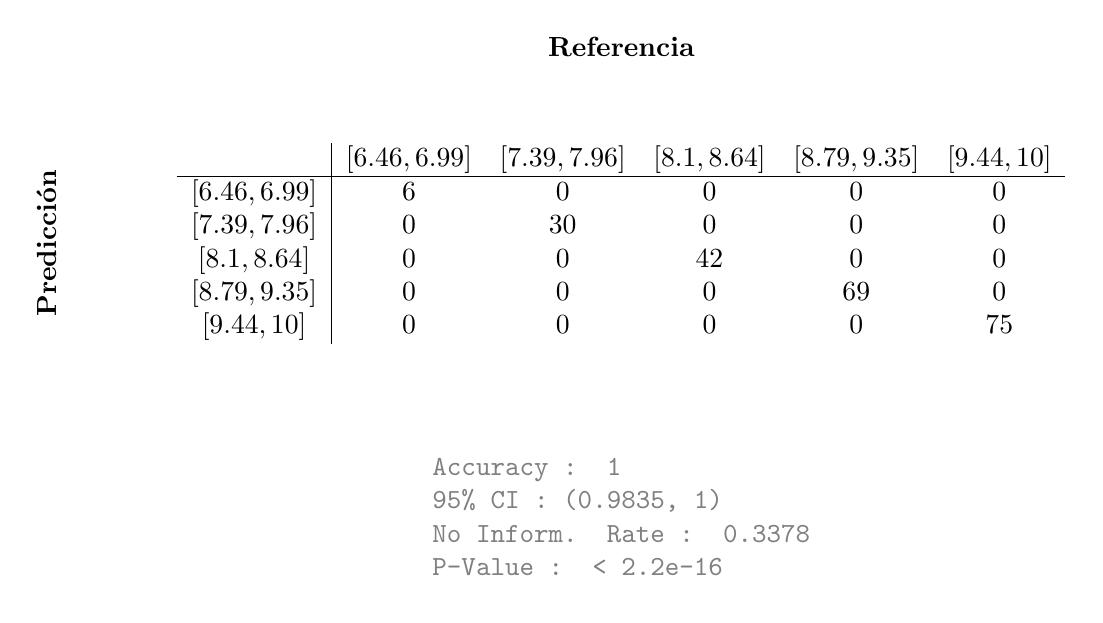
\begin{tikzpicture}
  \node (matrix)  {$\begin{array}{c|ccccc}
                         & \left[6.46,6.99\right] & \left[7.39,7.96\right] & \left[8.1,8.64\right] & \left[8.79,9.35\right] & \left[9.44,10\right]\\ \hline
        \left[6.46,6.99\right] & 6 & 0 & 0 & 0 & 0 \\
        \left[7.39,7.96\right] & 0 & 30 & 0 & 0 & 0 \\
        \left[8.1,8.64\right] & 0 & 0 & 42 & 0 & 0 \\
        \left[8.79,9.35\right] & 0 & 0 & 0 & 69 & 0 \\
        \left[9.44,10\right] & 0 & 0 & 0 & 0 & 75
\end{array}$};
  \node[above of= matrix, node distance=1.5cm, yshift=1cm,font=\color{black}] {\textbf{Referencia}};
  \node[left of= matrix, node distance=8cm, rotate=90, anchor=center,yshift=-0.7cm,font=\color{black}] {\textbf{Predicción}};
  % Tabular environment for additional text
  \node[below of=matrix, node distance=3.5cm,font=\color{gray}]{
    \begin{tabular}{l}
      \texttt{Accuracy : 1} \\
      \texttt{95\% CI : (0.9835, 1)} \\
      \texttt{No Inform. Rate : 0.3378} \\
      \texttt{P-Value : < 2.2e-16 }
    \end{tabular}
  };
\end{tikzpicture}
\caption{Aprendiendo a identificar a los grupos de prácticas con un intervalo de notas (Figura \ref{fig:KMeans5}).}
\label{fig:cmbegin2}
\end{figure}

\begin{tcolorbox}[title=Reglas de clasificación para identificar intervalos de notas.]
  %add special color box to list of listings
  \makeatletter
  \addcontentsline{lol}{subsection}{\kvtcb@title}
  \makeatother
\begin{multicols}{3}
    \begin{minted}[fontsize=\scriptsize]{R}
Rule 99/1: (3.5, lift 17.3)
	ot > 0.4421769
	ot <= 0.4642857
	ps > 0.1079545
	->  class [6.46,6.99]  [0.817]

Rule 99/2: (7.8/2.7, lift 13.2)
	ns <= 0.0450045
	sq <= 0.9528306
	->  class [6.46,6.99]  [0.624]

Rule 99/3: (10.8, lift 5.5)
	ns > 0.2360656
	ns <= 0.3171171
	rt > 0.008
	rt <= 0.03660131
	ps > 0.1712963
	->  class [7.39,7.96]  [0.922]

Rule 99/4: (7.6/0.5, lift 5.0)
	ns > 0.1616162
	ns <= 0.2083805
	ot > 0.4642857
	rt > 0.1785714
	ps > 0.008561644
	sq > 0.9268974
	->  class [7.39,7.96]  [0.840]

Rule 99/5: (7.7/1.2, lift 3.7)
	ns > 0.226087
	ns <= 0.2557377
	ot > 0.4642857
	rt > 0.03660131
	->  class [8.1,8.64]  [0.769]

Rule 99/6: (15.7/4, lift 3.4)
	ns <= 0.0450045
	sq > 0.9528306
	->  class [8.1,8.64]  [0.718]

Rule 99/7: (7.5/1.8, lift 3.4)
	ot > 0.4642857
	rt <= 0
	->  class [8.1,8.64]  [0.705]

Rule 99/8: (31.6/13.9, lift 2.7)
	ot <= 0.4642857
	ps <= 0.1079545
  ->  class [8.1,8.64] [0.558]

Rule 99/9: (38.4/23.6, lift 1.9)
	rt > 0.4194915
	->  class [8.1,8.64]  [0.390]

Rule 99/10: (6, lift 3.3)
	ns > 0.2083805
	rt > 0.03660131
	fr <= 0.1424242
	->  class [8.79,9.35]  [0.875]

Rule 99/11: (5.5, lift 3.3)
	ns > 0.4709596
	rt > 0.03660131
	rt <= 0.4194915
	->  class [8.79,9.35]  [0.866]

Rule 99/12: (5.3, lift 3.3)
	ns > 0.2557377
	st > 1.040305
	ps > 0.09157895
	->  class [8.79,9.35]  [0.863]

Rule 99/13: (15/1.3, lift 3.3)
	ns > 0.08820882
	ns <= 0.1616162
	ot > 0.4642857
	rt > 0.03660131
	rt <= 0.4194915
  ->  class [8.79,9.35] [0.862]

Rule 99/14: (3.2, lift 3.1)
	ns > 0.0450045
	ns <= 0.2083805
	ps <= 0.008561644
  ->  class [8.79,9.35] [0.809]

Rule 99/15: (12.1/4.1, lift 2.4)
	ns <= 0.2868852
	ot <= 0.4421769
	ps > 0.1079545
	sq <= 0.9877296
  ->  class [8.79,9.35] [0.637]

Rule 99/16: (6.6, lift 2.8)
	ns > 0.2868852
	ns <= 0.5189189
	ot <= 0.4642857
	ps > 0.1079545
	->  class [9.44,10]  [0.884]

Rule 99/17: (7.5/0.4, lift 2.7)
	ns <= 0.2083805
	ot > 0.4642857
	rt <= 0.4194915
	sq <= 0.9012999
	->  class [9.44,10]  [0.856]

Rule 99/18: (198.5/132, lift 1.1)
	ns > 0.0450045
	->  class [9.44,10]  [0.337]
	
Default class: [9.44,10]
    \end{minted}
  \end{multicols}
\label{rulesbegin2}
\end{tcolorbox}

\subsection{Clasificación empleando una combinación de todas las métricas}

A continuación, se repetirán los experimentos anteriores, pero ahora empleando las funciones $np$, $fr$, $ps$, $sq$, $Cl$, $De$, $Dm$, $Le$, $Di$, $We$, $Ef$, $St$, $Dag$, $WDag$, $Be$ y $Ba$.

\subsubsection{Clasificación empleando los niveles 8, 9 y 10}

Empleando el algoritmo C5.0 se obtiene un conjunto de reglas (Cuadro \ref{rules8}) capaz de clasificar exactamente todos los grupos dentro de su correspondiente intervalo de calificaciones del nivel $8$ en adelante, es decir, a partir del último tercio del periodo de tiempo dedicado a la práctica, con un $p$ value $p < 2.2e-16$ estadísticamente muy relevante (Figura \ref{fig:cm8}).

\begin{figure}[H]
\centering
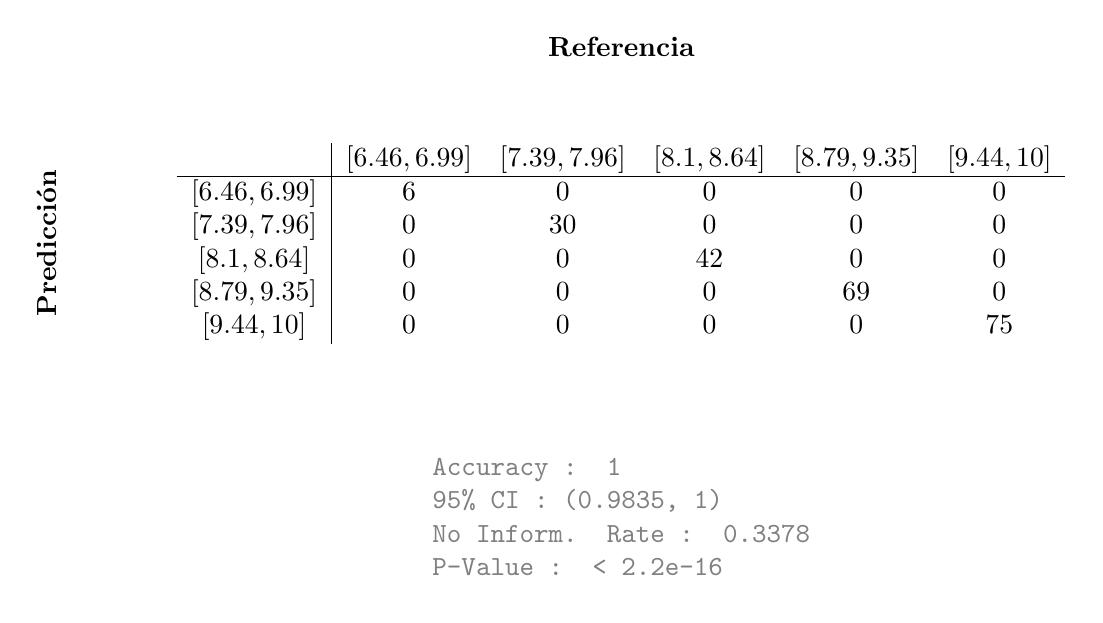
\begin{tikzpicture}
  \node (matrix)  {$\begin{array}{c|ccccc}
                         & \left[6.46,6.99\right] & \left[7.39,7.96\right] & \left[8.1,8.64\right] & \left[8.79,9.35\right] & \left[9.44,10\right]\\ \hline
        \left[6.46,6.99\right] & 6 & 0 & 0 & 0 & 0 \\
        \left[7.39,7.96\right] & 0 & 30 & 0 & 0 & 0 \\
        \left[8.1,8.64\right] & 0 & 0 & 42 & 0 & 0 \\
        \left[8.79,9.35\right] & 0 & 0 & 0 & 69 & 0 \\
        \left[9.44,10\right] & 0 & 0 & 0 & 0 & 75
\end{array}$};
  \node[above of= matrix, node distance=1.5cm, yshift=1cm,font=\color{black}] {\textbf{Referencia}};
  \node[left of= matrix, node distance=8cm, rotate=90, anchor=center,yshift=-0.7cm,font=\color{black}] {\textbf{Predicción}};
  % Tabular environment for additional text
  \node[below of=matrix, node distance=3.5cm,font=\color{gray}]{
    \begin{tabular}{l}
      \texttt{Accuracy : 1} \\
      \texttt{95\% CI : (0.9835, 1)} \\
      \texttt{No Inform. Rate : 0.3378} \\
      \texttt{P-Value : < 2.2e-16 }
    \end{tabular}
  };
\end{tikzpicture}
\caption{Aprendiendo a identificar a los grupos de prácticas con un intervalo de notas (Figura \ref{fig:KMeans5}).}
\label{fig:cm8}
\end{figure}

\begin{tcolorbox}[title=Reglas de clasificación para identificar intervalos de notas.]
  %add special color box to list of listings
  \makeatletter
  \addcontentsline{lol}{subsection}{\kvtcb@title}
  \makeatother
\begin{multicols}{3}
    \begin{minted}[fontsize=\scriptsize]{R}
Rule 99/1: (9.5/0.4, lift 21.4)
	sq > 0.9411765
	sq <= 0.9693
	We <= 0.320432
	WDag > -4.46152
	->  class [6.46,6.99]  [0.875]

Rule 99/2: (187.1/143.7, lift 1.2)
	Be <= 6
	->  class [7.39,7.96]  [0.235]

Rule 99/3: (10.2/1.7, lift 4.2)
	ps <= 0.09064327
	sq > 0.9693
	Dag <= -5.723585
	Be <= 6
	Ba > 6.97672
	->  class [8.1,8.64]  [0.781]

Rule 99/4: (10.8/1.9, lift 4.2)
	sq > 0.9693
	Cl > 0.2
	We <= 0.1530153
	Be <= 6
	->  class [8.1,8.64]  [0.772]

Rule 99/5: (13.6/3.5, lift 3.8)
	Cl > 0.2083333
	Be <= 1
	->  class [8.1,8.64]  [0.711]

Rule 99/6: (5.3/1.4, lift 3.6)
	sq <= 0.9411765
	Cl <= 0.1343604
	Be <= 6
	->  class [8.1,8.64]  [0.675]

Rule 99/7: (9, lift 3.1)
	fr > 0.07135135
	ps > 0.07638889
	sq > 0.9693
	Cl <= 0.1656004
	Be <= 6
	Ba <= 6.97672
	->  class [8.79,9.35]  [0.909]

Rule 99/8: (6.2, lift 3.0)
	We > 0.8504505
	Be > 6
	->  class [8.79,9.35]  [0.878]

Rule 99/9: (14.5/1.2, lift 3.0)
	ps <= 0.09064327
	sq > 0.9693
	Le <= -8.25175
	Ef > 7
	Dag > -5.723585
	Ba > 6.97672
	->  class [8.79,9.35]  [0.864]

Rule 99/10: (22.1/3.2, lift 2.8)
	sq <= 0.9411765
	Cl > 0.1343604
	Cl <= 0.2083333
   ->  class [8.79,9.35] [0.825]

Rule 99/11: (5.3/0.8, lift 2.6)
	fr <= 0.04105572
	sq > 0.9938784
	Ef > 7
	->  class [8.79,9.35]  [0.758]

Rule 99/12: (5.7/1.5, lift 2.3)
	We <= 0.2364532
	Be > 6
	->  class [8.79,9.35]  [0.673]

Rule 99/13: (11.4/4.6, lift 2.0)
	sq > 0.9693
	Ba > 9.917424
  ->  class [8.79,9.35] [0.586]

Rule 99/14: (13.6, lift 3.3)
	sq <= 0.9411765
	Cl > 0.2083333
	Be > 1
	->  class [9.44,10]  [0.936]

Rule 99/15: (5.3, lift 3.1)
	fr <= 0.04105572
	sq > 0.9693
	sq <= 0.9938784
	Le > -8.25175
	We > 0.1530153
	->  class [9.44,10]  [0.863]

Rule 99/16: (11.9/1.4, lift 2.9)
	sq > 0.9693
	Cl > 0.1656004
	Le <= -8.25175
	We > 0.1530153
	Ba <= 6.97672
	->  class [9.44,10]  [0.829]

Rule 99/17: (8.6/1.6, lift 2.7)
	sq > 0.9411765
	sq <= 0.9693
	We > 0.320432
	WDag > -4.46152
	->  class [9.44,10]  [0.759]

Rule 99/18: (23.1/5.1, lift 2.7)
	We > 0.2364532
	We <= 0.8504505
	Be > 6
	->  class [9.44,10]  [0.757]
	
Default class: [8.79,9.35]
    \end{minted}
  \end{multicols}
\label{rules8}
\end{tcolorbox}

\subsubsection{Clasificación empleando los niveles 3, 4 y 5}

Al igual que en el caso anterior, empleando el algoritmo C5.0 obtenemos un conjunto de reglas (Cuadro \ref{rules7}) capaz de clasificar exactamente todos los grupos dentro de su correspondiente intervalo de calificaciones del nivel $3$ al $5$, es decir, a partir del primer tercio del periodo de tiempo dedicado a la práctica, con un $p$ value $p < 2.2e-16$ estadísticamente muy relevante (Figura \ref{fig:cm7}).

\begin{figure}[H]
\centering
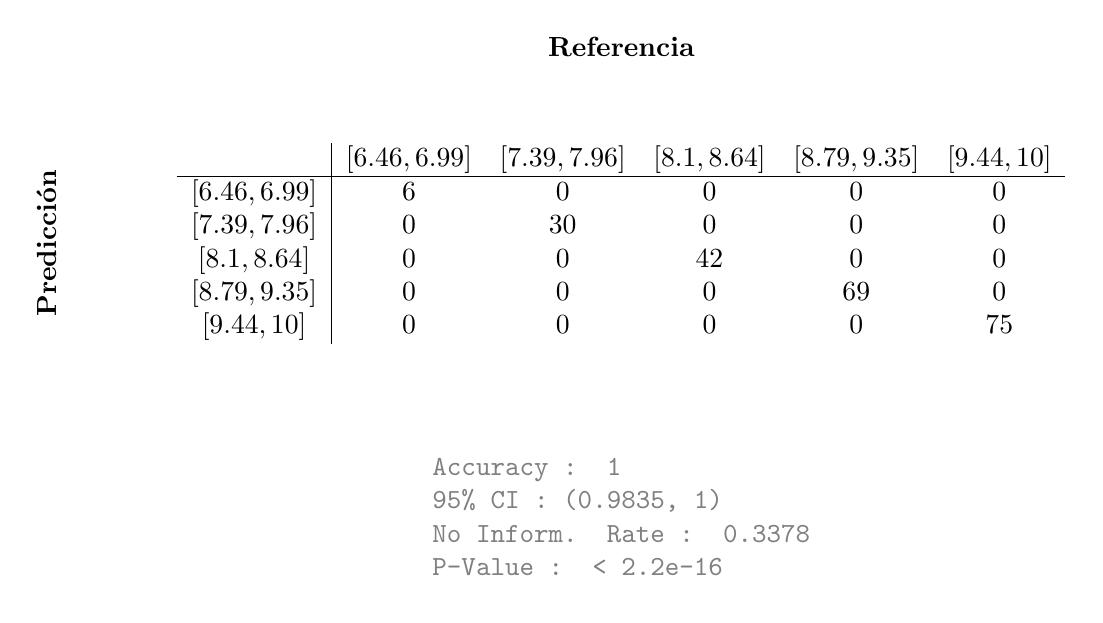
\begin{tikzpicture}
  \node (matrix)  {$\begin{array}{c|ccccc}
                         & \left[6.46,6.99\right] & \left[7.39,7.96\right] & \left[8.1,8.64\right] & \left[8.79,9.35\right] & \left[9.44,10\right]\\ \hline
        \left[6.46,6.99\right] & 6 & 0 & 0 & 0 & 0 \\
        \left[7.39,7.96\right] & 0 & 30 & 0 & 0 & 0 \\
        \left[8.1,8.64\right] & 0 & 0 & 42 & 0 & 0 \\
        \left[8.79,9.35\right] & 0 & 0 & 0 & 69 & 0 \\
        \left[9.44,10\right] & 0 & 0 & 0 & 0 & 75
\end{array}$};
  \node[above of= matrix, node distance=1.5cm, yshift=1cm,font=\color{black}] {\textbf{Referencia}};
  \node[left of= matrix, node distance=8cm, rotate=90, anchor=center,yshift=-0.7cm,font=\color{black}] {\textbf{Predicción}};
  % Tabular environment for additional text
  \node[below of=matrix, node distance=3.5cm,font=\color{gray}]{
    \begin{tabular}{l}
      \texttt{Accuracy : 1} \\
      \texttt{95\% CI : (0.9835, 1)} \\
      \texttt{No Inform. Rate : 0.3378} \\
      \texttt{P-Value : < 2.2e-16 }
    \end{tabular}
  };
\end{tikzpicture}
\caption{Aprendiendo a identificar a los grupos de prácticas con un intervalo de notas (Figura \ref{fig:KMeans5}).}
\label{fig:cm7}
\end{figure}

\begin{tcolorbox}[title=Reglas de clasificación para identificar intervalos de notas.]
  %add special color box to list of listings
  \makeatletter
  \addcontentsline{lol}{subsection}{\kvtcb@title}
  \makeatother
\begin{multicols}{3}
    \begin{minted}[fontsize=\scriptsize]{R}
Rule 99/1: (2.7, lift 21.1)
	sq <= 0.9622505
	Cl > 0.5666667
	We <= 0.06544687
	Dag > -4.49981
  ->  class [6.46,6.99] [0.788]

Rule 99/2: (7.3/1.8, lift 18.8)
	We <= 0.1574179
	Dag <= -5.049856
	Ba > 7.302562
	->  class [6.46,6.99]  [0.705]

Rule 99/3: (7.5, lift 5.3)
	ps <= 0.1712963
	sq > 0.9964787
	We <= 0.06544687
	St <= 0
	->  class [7.39,7.96]  [0.894]

Rule 99/4: (2.8, lift 4.6)
	ps <= 0.04761905
	We <= 0.1945946
	WDag <= -6.625771
	->  class [7.39,7.96]  [0.791]

Rule 99/5: (2.7, lift 4.6)
	sq <= 0.9622505
	We <= 0.06544687
	Dag <= -4.49981
	->  class [7.39,7.96]  [0.785]

Rule 99/6: (4.5/0.5, lift 4.5)
	sq > 0.9622505
	We > 0.02880288
	We <= 0.06544687
	St <= 0
	->  class [7.39,7.96]  [0.768]

Rule 99/7: (6.3/1.5, lift 4.1)
	Cl <= 0.2307692
	We > 0.1574179
	We <= 0.4671717
	Dag <= -5.049856
	->  class [7.39,7.96]  [0.705]

Rule 99/8: (9.7, lift 4.1)
	ps <= 0.1712963
	sq > 0.9622505
	sq <= 0.9964787
	We <= 0.02880288
	->  class [8.1,8.64]  [0.914]

Rule 99/9: (7.6, lift 4.0)
	fr <= 0.05555556
  ->  class [8.1,8.64] [0.896]

Rule 99/10: (5.8, lift 3.9)
	ps <= 0.1712963
	sq > 0.9622505
	We <= 0.06544687
	St > 0
	->  class [8.1,8.64]  [0.872]

Rule 99/11: (3.3, lift 3.7)
	Cl > 0.7222222
	We > 0.06544687
	->  class [8.1,8.64]  [0.811]

Rule 99/12: (9.1/1.5, lift 3.5)
	ps <= 0.04761905
	We > 0.1945946
	Dag > -5.049856
	->  class [8.1,8.64]  [0.779]

Rule 99/13: (7.1/1.6, lift 3.2)
	Cl > 0.2307692
	We > 0.1574179
	We <= 0.4671717
	Dag <= -5.049856
	->  class [8.1,8.64]  [0.709]

Rule 99/14: (10.3, lift 3.5)
	ps <= 0.04761905
	Cl <= 0.7222222
	We > 0.06544687
	We <= 0.1945946
	WDag > -6.625771
	->  class [8.79,9.35]  [0.919]

Rule 99/15: (7, lift 3.3)
	ps > 0.09866667
	sq > 0.9811558
	Cl <= 0.5238096
	Be <= 1
	->  class [8.79,9.35]  [0.888]

Rule 99/16: (4.3, lift 3.2)
	ps > 0.1311475
	Dag > -5.049856
	Be > 3
  ->  class [8.79,9.35] [0.840]

Rule 99/17: (4, lift 3.1)
	ps > 0.04761905
	ps <= 0.2626263
	Le > -4.49981
  ->  class [8.79,9.35] [0.834]

Rule 99/18: (20.1/3.6, lift 3.0)
	ps > 0.09866667
	ps <= 0.2626263
	sq <= 0.9811558
	Cl <= 0.5833333
	We > 0.06544687
	Dag > -5.049856
	Ba <= 8.242092
  ->  class [8.79,9.35] [0.792]

Rule 99/19: (176.2/118.8, lift 1.2)
	We > 0.06544687
  ->  class [8.79,9.35] [0.328]

Rule 99/20: (4.8, lift 2.8)
	sq <= 0.9622505
	Cl <= 0.5666667
	We <= 0.06544687
	->  class [9.44,10]  [0.853]

Rule 99/21: (19.7/6.2, lift 2.2)
	fr > 0.1818182
	Cl > 0.2619048
	Di <= -4.219508
	Be > 1
	Ba <= 5.211599
	->  class [9.44,10]  [0.671]

Rule 99/22: (145.2/87.7, lift 1.3)
	We > 0.06544687
	Dag > -5.049856
	->  class [9.44,10]  [0.398]
	
Default class: [8.79,9.35]
    \end{minted}
  \end{multicols}
\label{rules7}
\end{tcolorbox}

\subsection{Clasificación empleando las medidas de complejidad de propósito general}

\subsubsection{Clasificación empleando los niveles 8, 9 y 10}

Empleando el algoritmo C5.0 obtenemos un conjunto de reglas (Cuadro \ref{rules6}) capaz de clasificar exactamente todos los grupos dentro de su correspondiente intervalo de calificaciones del nivel $8$ en adelante, es decir, a partir del último tercio del periodo de tiempo dedicado a la práctica, con un $p$ value $p < 2.2e-16$ estadísticamente muy relevante (Figura \ref{fig:cm6}).

\begin{figure}[H]
\centering
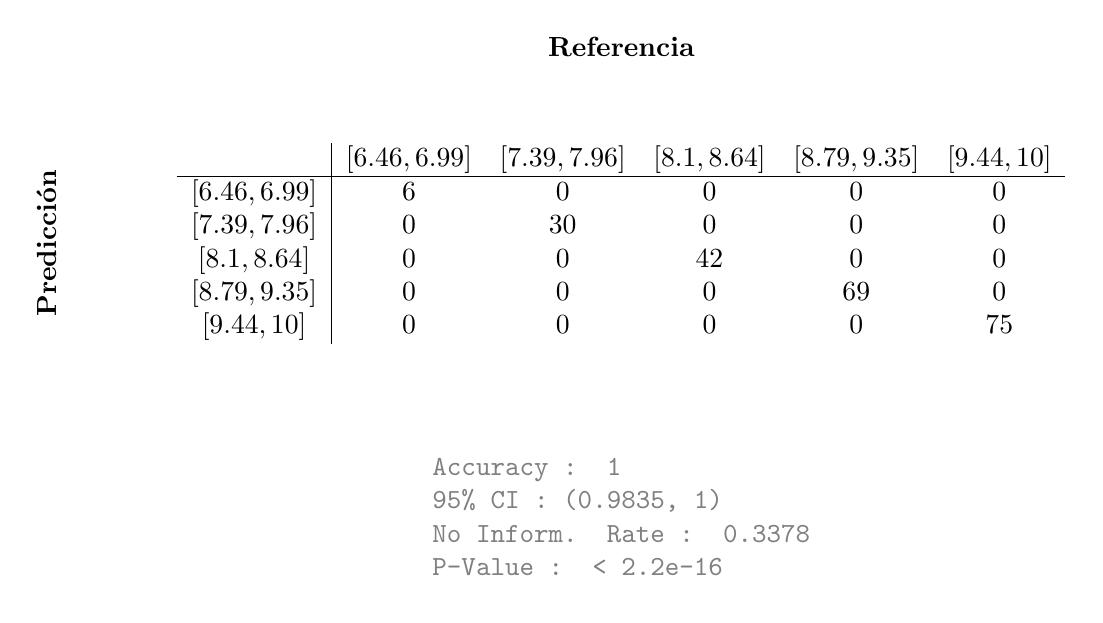
\begin{tikzpicture}
  \node (matrix)  {$\begin{array}{c|ccccc}
                         & \left[6.46,6.99\right] & \left[7.39,7.96\right] & \left[8.1,8.64\right] & \left[8.79,9.35\right] & \left[9.44,10\right]\\ \hline
        \left[6.46,6.99\right] & 6 & 0 & 0 & 0 & 0 \\
        \left[7.39,7.96\right] & 0 & 30 & 0 & 0 & 0 \\
        \left[8.1,8.64\right] & 0 & 0 & 42 & 0 & 0 \\
        \left[8.79,9.35\right] & 0 & 0 & 0 & 69 & 0 \\
        \left[9.44,10\right] & 0 & 0 & 0 & 0 & 75
\end{array}$};
  \node[above of= matrix, node distance=1.5cm, yshift=1cm,font=\color{black}] {\textbf{Referencia}};
  \node[left of= matrix, node distance=8cm, rotate=90, anchor=center,yshift=-0.7cm,font=\color{black}] {\textbf{Predicción}};
  % Tabular environment for additional text
  \node[below of=matrix, node distance=3.5cm,font=\color{gray}]{
    \begin{tabular}{l}
      \texttt{Accuracy : 1} \\
      \texttt{95\% CI : (0.9835, 1)} \\
      \texttt{No Inform. Rate : 0.3378} \\
      \texttt{P-Value : < 2.2e-16 }
    \end{tabular}
  };
\end{tikzpicture}
\caption{Aprendiendo a identificar a los grupos de prácticas con un intervalo de notas (Figura \ref{fig:KMeans5}).}
\label{fig:cm6}
\end{figure}

\begin{tcolorbox}[title=Reglas de clasificación para identificar intervalos de notas.]
  %add special color box to list of listings
  \makeatletter
  \addcontentsline{lol}{subsection}{\kvtcb@title}
  \makeatother
\begin{multicols}{3}
    \begin{minted}[fontsize=\scriptsize]{R}
Rule 99/1: (7.5/2.7, lift 17.2)
	We <= 0.3132313
	Dag > -5.834811
	Dag <= -5.723585
	WDag > -4.46152
	Ba > 6.97672
  ->  class [6.46,6.99] [0.614]

Rule 99/2: (5.6, lift 5.5)
	Dm > 1.142857
	We > 0.3132313
	St <= 3.988984
	Ba > 5.625386
	->  class [7.39,7.96]  [0.868]

Rule 99/3: (5.1, lift 5.5)
	De > 0.09558824
	We <= 0.3132313
	Dag <= -5.723585
	WDag <= -4.46152
  ->  class [7.39,7.96] [0.859]

Rule 99/4: (8.7/1.1, lift 5.1)
	Dm > 1.142857
	Di > -7.196687
	We <= 0.3132313
	Be <= 5
	Ba > 5.351235
	->  class [7.39,7.96]  [0.805]

Rule 99/5: (4.4/1.2, lift 4.2)
	Cl <= 0.1688889
	Le > -8.98097
	Be <= 1
	->  class [7.39,7.96]  [0.653]

Rule 99/6: (5.3, lift 4.1)
	Dm > 1.142857
	We <= 0.3132313
	Ef > 7
	WDag <= -3.011829
	Ba <= 5.351235
	->  class [8.1,8.64]  [0.863]

Rule 99/7: (18.5/3.6, lift 3.7)
	De > 0.1169591
	Dag <= -5.605802
	Be > 1
	Be <= 6
	Ba > 6.97672
  ->  class [8.1,8.64] [0.777]

Rule 99/8: (9.6/1.6, lift 3.7)
	De > 0.1535948
	Ba > 5.351235
	Ba <= 6.97672
	->  class [8.1,8.64]  [0.772]

Rule 99/9: (9.4/2.3, lift 3.4)
	Dm <= 1.071429
	Ba <= 6.776386
	->  class [8.1,8.64]  [0.711]

Rule 99/10: (190.3/128.8, lift 1.1)
	Dm > 1.142857
  ->  class [8.79,9.35] [0.325]

Rule 99/11: (9, lift 3.1)
	De <= 0.1169591
	Dm > 1.588235
	We > 0.3132313
	Ba > 6.036998
	->  class [9.44,10]  [0.909]

Rule 99/12: (18/1, lift 3.0)
	Cl > 0.1611913
	Cl <= 0.2582892
	De <= 0.1169591
	We > 0.3132313
	St > 3.988984
	->  class [9.44,10]  [0.898]

Rule 99/13: (6.7, lift 3.0)
	We <= 0.3132313
	Dag > -5.834811
	WDag > -3.011829
	->  class [9.44,10]  [0.885]

Rule 99/14: (4.1, lift 2.8)
	Dm > 1.142857
	We > 0.3132313
	Ba > 4.849921
	Ba <= 5.351235
	->  class [9.44,10]  [0.836]

Rule 99/15: (10.2/1.8, lift 2.6)
	De > 0.1169591
	De <= 0.1535948
	We > 0.3132313
	Dag <= -5.605802
	Ba <= 6.97672
	->  class [9.44,10]  [0.767]

Rule 99/16: (16.3/3.4, lift 2.6)
	Dm <= 1.142857
	Ba > 6.776386
	->  class [9.44,10]  [0.757]

Rule 99/17: (13.3/4.7, lift 2.1)
	Dm > 1.071429
	Dm <= 1.142857
	->  class [9.44,10]  [0.625]

Default class: [8.79,9.35]
    \end{minted}
  \end{multicols}
\label{rules6}
\end{tcolorbox}

\subsubsection{Clasificación empleando los niveles 3, 4 y 5}

Efectivamente, C5.0 obtiene un conjunto de reglas (Cuadro \ref{rules5}) capaz de clasificar exactamente todos los grupos dentro de su correspondiente intervalo de calificaciones del nivel $3$ en adelante, es decir, a partir de un tercio del periodo de tiempo dedicado a la práctica, con un $p$ value $p < 2.2e-16$ estadísticamente muy relevante (Figura \ref{fig:cm5}).

\begin{figure}[H]
\centering
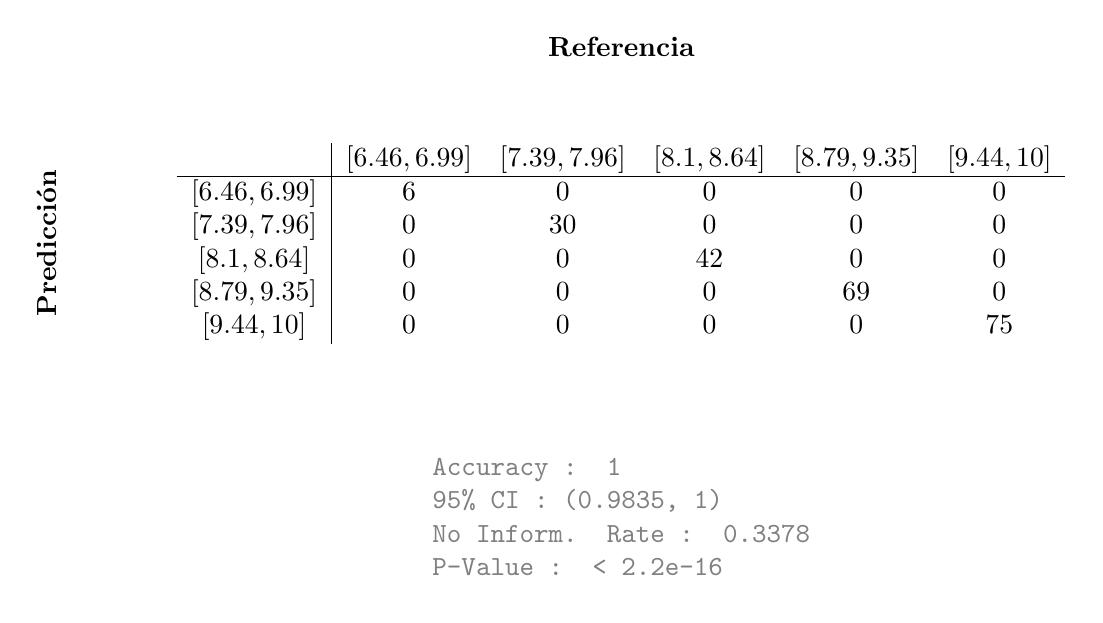
\begin{tikzpicture}
  \node (matrix)  {$\begin{array}{c|ccccc}
                         & \left[6.46,6.99\right] & \left[7.39,7.96\right] & \left[8.1,8.64\right] & \left[8.79,9.35\right] & \left[9.44,10\right]\\ \hline
        \left[6.46,6.99\right] & 6 & 0 & 0 & 0 & 0 \\
        \left[7.39,7.96\right] & 0 & 30 & 0 & 0 & 0 \\
        \left[8.1,8.64\right] & 0 & 0 & 42 & 0 & 0 \\
        \left[8.79,9.35\right] & 0 & 0 & 0 & 69 & 0 \\
        \left[9.44,10\right] & 0 & 0 & 0 & 0 & 75
\end{array}$};
  \node[above of= matrix, node distance=1.5cm, yshift=1cm,font=\color{black}] {\textbf{Referencia}};
  \node[left of= matrix, node distance=8cm, rotate=90, anchor=center,yshift=-0.7cm,font=\color{black}] {\textbf{Predicción}};
  % Tabular environment for additional text
  \node[below of=matrix, node distance=3.5cm,font=\color{gray}]{
    \begin{tabular}{l}
      \texttt{Accuracy : 1} \\
      \texttt{95\% CI : (0.9835, 1)} \\
      \texttt{No Inform. Rate : 0.3378} \\
      \texttt{P-Value : < 2.2e-16 }
    \end{tabular}
  };
\end{tikzpicture}
\caption{Aprendiendo a identificar a los grupos de prácticas con un intervalo de notas (Figura \ref{fig:KMeans5}).}
\label{fig:cm5}
\end{figure}

\begin{tcolorbox}[title=Reglas de clasificación para identificar intervalos de notas.]
  %add special color box to list of listings
  \makeatletter
  \addcontentsline{lol}{subsection}{\kvtcb@title}
  \makeatother
\begin{multicols}{3}
    \begin{minted}[fontsize=\scriptsize]{R}
Rule 99/1: (4.6, lift 4.7)
	We <= 0.01080108
	Ba > 3.366005
	->  class [7.39,7.96]  [0.848]

Rule 99/2: (3.4, lift 4.5)
	We <= 0.2018018
	WDag <= -6.478509
	Be <= 1
	->  class [7.39,7.96]  [0.815]

Rule 99/3: (9.4/2.2, lift 4.0)
	We <= 0.2702703
	St > 1.791759
	St <= 2.079442
	->  class [7.39,7.96]  [0.721]

Rule 99/4: (11.1/3.5, lift 3.6)
	Cl > 0.2619048
	Di <= -4.219508
	We > 0.2131148
	We <= 0.2702703
	St > 0
	WDag <= -5.901418
	->  class [7.39,7.96]  [0.653]

Rule 99/5: (6.5/2.1, lift 3.5)
	De <= 0.0952381
	We <= 0.1321739
  ->  class [7.39,7.96] [0.630]

Rule 99/6: (10.2/6.1, lift 2.3)
	St > 5.257495
	->  class [7.39,7.96]  [0.414]

Rule 99/7: (7.6/0.5, lift 3.6)
	We > 0.2702703
	St <= 0
	WDag > -7.122867
  ->  class [8.1,8.64] [0.840]

Rule 99/8: (4.1, lift 3.6)
	We <= 0.2702703
	St > 2.079442
	WDag <= -5.296464
	Be <= 2
	->  class [8.1,8.64]  [0.837]

Rule 99/9: (9.4/1.8, lift 3.2)
	Cl > 0.4095238
	We <= 0.2702703
	St > 0
	St <= 1.791759
	Dag > -5.204007
	Ba > 5.925958
	->  class [8.1,8.64]  [0.751]

Rule 99/10: (6.3/1.9, lift 2.8)
	De <= 0.0952381
	We > 0.1321739
	->  class [8.1,8.64]  [0.658]

Rule 99/11: (17.1/6, lift 2.7)
	De > 0.0952381
	We > 0.01080108
	We <= 0.04410441
	Ba > 3.366005
	->  class [8.1,8.64]  [0.633]

Rule 99/12: (6.7/2.3, lift 2.7)
	We <= 0.01080108
	Ba <= 3.366005
	->  class [8.1,8.64]  [0.621]

Rule 99/13: (187.3/131.4, lift 1.1)
	We > 0.04410441
	->  class [8.79,9.35]  [0.301]

Rule 99/14: (9.2, lift 3.1)
	Cl > 0.2619048
	Di <= -4.219508
	We > 0.1415628
	We <= 0.2131148
	St > 0
	St <= 2.079442
	Ba <= 5.925958
	->  class [9.44,10]  [0.911]

Rule 99/15: (7.1, lift 3.0)
	We > 0.2018018
	We <= 0.2287122
	St <= 0
	->  class [9.44,10]  [0.890]

Rule 99/16: (6.8, lift 3.0)
	We > 0.2702703
	St <= 0
	WDag > -8.251143
	WDag <= -7.122867
	->  class [9.44,10]  [0.886]

Rule 99/17: (5.5, lift 2.9)
	We > 0.2131148
	St <= 2.079442
	WDag > -5.901418
	->  class [9.44,10]  [0.867]

Rule 99/18: (5.1, lift 2.9)
	We > 0.01080108
	We <= 0.04410441
	Ba <= 3.366005
	->  class [9.44,10]  [0.860]

Rule 99/19: (4.7, lift 2.9)
	We > 0.04410441
	St <= 0
	WDag > -5.755742
	->  class [9.44,10]  [0.851]

Rule 99/20: (11.5/1.3, lift 2.8)
	Dm <= 1
	Di <= -4.219508
	We > 0.04410441
	We <= 0.2131148
	St > 0
	Ba <= 5.925958
	->  class [9.44,10]  [0.832]

Rule 99/21: (9.1/1.7, lift 2.6)
	Cl > 0.2792208
	We > 0.2702703
	St > 1.386294
	Dag > -5.204007
	Be > 1
	->  class [9.44,10]  [0.759]

Rule 99/22: (10.6/2.6, lift 2.4)
	Cl <= 0.4095238
	De > 0.0952381
	St <= 1.791759
	Be > 2
	Ba > 5.925958
	->  class [9.44,10]  [0.718]

Default class: [9.44,10]
    \end{minted}
  \end{multicols}
\label{rules5}
\end{tcolorbox}